% Slide 07 — the one loud thing.
% The whole design rests on this: everything else on the screen stays quiet so
% that a single prohibited finding is unmistakable. One red row in a field of
% grey, annotated with where the finding came from — drug, class, protocol.
\documentclass[border=0pt]{standalone}
% Figure preamble: the shared base plus a transparent page background, so a
% figure composites onto the slide ground instead of carrying a white box.
% Shared preamble for every Reconmed figure and slide.
\usepackage{xcolor}
\usepackage{graphicx}
\usepackage{tikz}
\usetikzlibrary{positioning,calc,fit,backgrounds,shapes.misc,arrows.meta,decorations.pathreplacing}

% Reconmed — presentation palette.
%
% A green medical theme, derived from the product's tokens (frontend/src/styles/
% tokens.css) but with the brand moved to a deep clinical green.
%
% The product's colour rule survives the rebrand unchanged: warm hues (alarm,
% caution) are reserved for prohibited findings and low confidence — never for
% change types. Change types stay cool and are kept off the brand green so the
% brand and the "add" state do not blur together.
\definecolor{ground}{HTML}{EFF4F0}
\definecolor{surf}{HTML}{FFFFFF}
\definecolor{surfii}{HTML}{F6FAF7}
\definecolor{surfiii}{HTML}{E5EDE7}

\definecolor{line}{HTML}{DBE5DD}
\definecolor{lineii}{HTML}{C1D1C4}
\definecolor{lineiii}{HTML}{92A796}

\definecolor{ink}{HTML}{10231A}
\definecolor{inkii}{HTML}{3B4F43}
\definecolor{inkiii}{HTML}{66796D}
\definecolor{inkiv}{HTML}{92A796}

% the brand green
\definecolor{brand}{HTML}{14532D}
\definecolor{brandii}{HTML}{1B6B3A}
\definecolor{brandwash}{HTML}{E8F2EA}

% the participant side of the call — cool and neutral, so the agent's green
% is the only brand colour on the slide
\definecolor{patient}{HTML}{4E6570}

% change types — cool, deliberately unalarming
\definecolor{add}{HTML}{15803D}
\definecolor{stop}{HTML}{6A4C93}
\definecolor{modify}{HTML}{1F5FA8}
\definecolor{same}{HTML}{6B7C70}

% the one loud thing
\definecolor{alarm}{HTML}{C2190B}
\definecolor{alarmink}{HTML}{A3170C}
\definecolor{alarmdim}{HTML}{F1B9B2}
\definecolor{alarmwash}{HTML}{FDF3F1}

% low confidence — dim gold, never red
\definecolor{caution}{HTML}{8A6206}

\definecolor{accept}{HTML}{15803D}
% Rejected is a decision, not an alarm: kept neutral so red stays reserved for
% prohibited findings.
\definecolor{reject}{HTML}{5F6B72}

% Type for the deck.
%
% Two families: Montserrat for headings, big numbers and the wordmark — a
% geometric sans that reads as a health brand — over Open Sans for everything
% else. Keeping the body on Open Sans matters: the dense technical slides were
% measured against it, so the small type does not reflow under the rebrand.
\usepackage{fontspec}
\defaultfontfeatures{Ligatures=TeX}
\setsansfont{Open Sans}
\newfontfamily\displayfont{Montserrat}
\renewcommand{\familydefault}{\sfdefault}

% Shared TikZ styles. Every figure draws in millimetres (x=1mm,y=1mm) on a
% 160x90 canvas, so these sizes are literal.
%
% No blank lines may appear inside the \tikzset below: a blank line is \par,
% and the key parser will not tolerate it.
\tikzset{
  panel/.style     = {draw=line, fill=surf,   line width=0.4pt, rounded corners=2pt},
  panelgray/.style = {draw=line, fill=surfii, line width=0.4pt, rounded corners=2pt},
  screen/.style    = {draw=line, fill=surf,   line width=0.5pt, rounded corners=2.5pt},
  hair/.style      = {draw=line,   line width=0.4pt},
  hairii/.style    = {draw=lineii, line width=0.5pt},
  dimbar/.style    = {fill=line,   rounded corners=0.6pt},
  dimbarsm/.style  = {fill=lineii, rounded corners=0.5pt},
  lab/.style       = {font=\fontsize{7}{8.5}\selectfont\sffamily\color{inkiii}, inner sep=0pt, outer sep=0pt},
  val/.style       = {font=\fontsize{9}{11}\selectfont\sffamily\color{ink},    inner sep=0pt, outer sep=0pt},
  valb/.style      = {font=\fontsize{9}{11}\selectfont\sffamily\bfseries\color{ink}, inner sep=0pt, outer sep=0pt},
  code/.style      = {font=\fontsize{7}{8.5}\selectfont\ttfamily\color{inkiii}, inner sep=0pt, outer sep=0pt},
  tag/.style       = {font=\fontsize{5.6}{6.5}\selectfont\sffamily\bfseries, inner xsep=1.3mm, inner ysep=0.7mm, rounded corners=1.4pt},
  pill/.style      = {font=\fontsize{6.4}{7.5}\selectfont\sffamily\bfseries, inner xsep=1.5mm, inner ysep=0.85mm, rounded corners=1.5pt},
  headline/.style  = {font=\fontsize{12}{14}\selectfont\sffamily\bfseries\color{ink}, anchor=west, inner sep=0pt, outer sep=0pt},
  subline/.style   = {font=\fontsize{7.5}{9}\selectfont\sffamily\color{inkii}, anchor=west, inner sep=0pt, outer sep=0pt},
  cardlab/.style   = {font=\fontsize{6.4}{7.5}\selectfont\sffamily\color{inkiii}, anchor=west, inner sep=0pt, outer sep=0pt},
  num/.style       = {font=\fontsize{22}{23}\selectfont\sffamily\bfseries\color{ink}, anchor=west, inner sep=0pt, outer sep=0pt},
  flow/.style      = {-{Stealth[length=1.5mm,width=1.2mm]}, draw=lineii, line width=0.7pt},
}

% The conmed mark.
%
% Concept: two records — the log on file, and what the participant said —
% converging into a single reconciled line. Drawn once as a standalone asset
% (shared/marks/conmed.tex) so it scales cleanly: PDF inclusion scales the
% strokes, which TikZ scope scaling would not.
\newcommand{\conmedmark}[1][16mm]{
\includegraphics[height=#1]{shared/marks/conmed.pdf}}


\AtBeginDocument{\ifdefined\nopagecolor\nopagecolor\fi}

\begin{document}
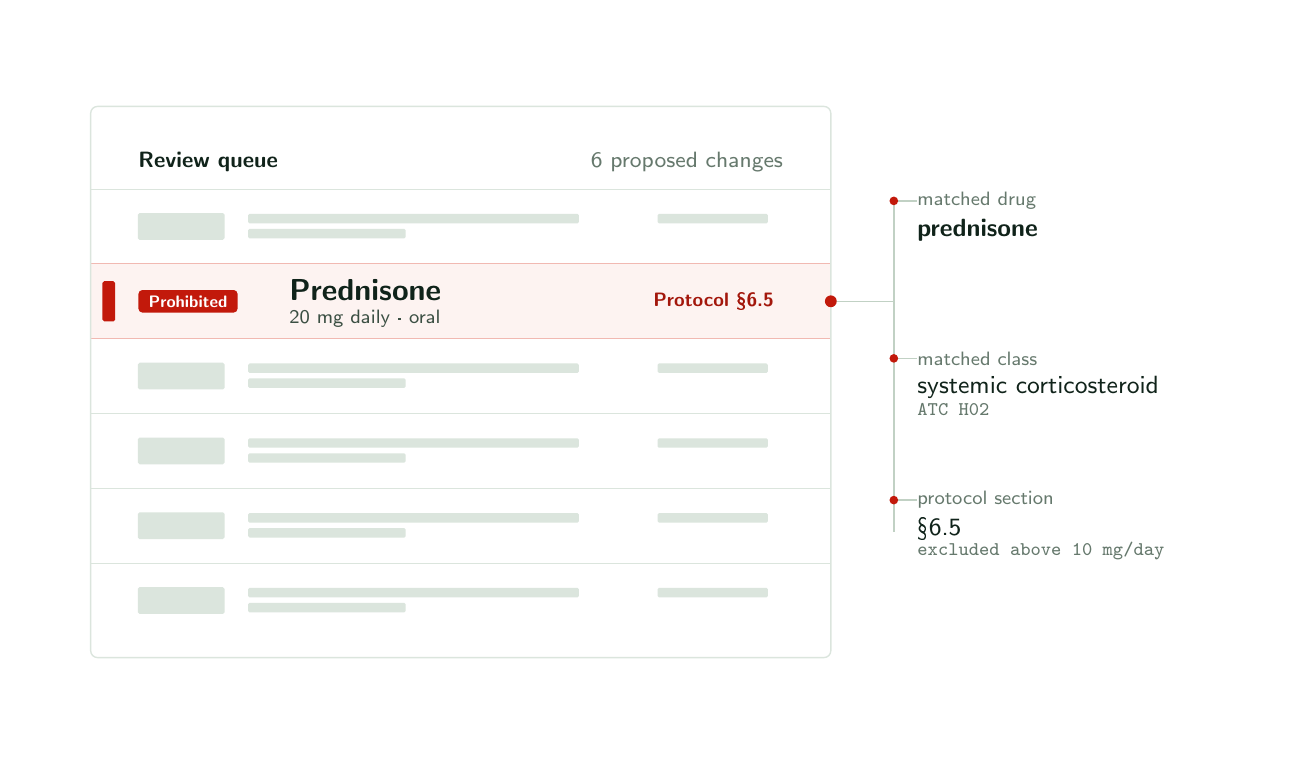
\begin{tikzpicture}[x=1mm,y=1mm]
\path[use as bounding box] (0,0) rectangle (160,90);

% a ghost of every other row: grey, quiet, unremarkable
\tikzset{
  ghostrow/.pic={
    \fill[line,   rounded corners=0.6pt] (0,-1.7)  rectangle (11,1.7);
    \fill[line,   rounded corners=0.5pt] (14,0.4)  rectangle (56,1.6);
    \fill[line,   rounded corners=0.5pt] (14,-1.5) rectangle (34,-0.3);
    \fill[line,   rounded corners=0.5pt] (66,0.4)  rectangle (80,1.6);
  }
}

% ---------- the review screen -------------------------------------------
\fill[surf, rounded corners=2.5pt] (8,10) rectangle (102,80);

% the one row that fires
\begin{scope}
  \clip[rounded corners=2.5pt] (8,10) rectangle (102,80);
  \fill[alarmwash] (8,50.5) rectangle (102,60);
\end{scope}

% row separators
\draw[line]      (8,60)   -- (102,60);
\draw[alarmdim]  (8,60)   -- (102,60);
\draw[alarmdim]  (8,50.5) -- (102,50.5);
\draw[line]      (8,41)   -- (102,41);
\draw[line]      (8,31.5) -- (102,31.5);
\draw[line]      (8,22)   -- (102,22);

% screen outline, on top of the fills
\draw[line, line width=0.5pt, rounded corners=2.5pt] (8,10) rectangle (102,80);

% header
\node[anchor=west, inner sep=0pt] at (14,73)
  {\fontsize{8.5}{10}\selectfont\sffamily\bfseries\color{ink} Review queue};
\node[anchor=east, inner sep=0pt] at (96,73)
  {\fontsize{8}{9}\selectfont\sffamily\color{inkiii} 6 proposed changes};
\draw[line] (8,69.5) -- (102,69.5);

% quiet rows
\pic at (14,64.75) {ghostrow};
\pic at (14,45.75) {ghostrow};
\pic at (14,36.25) {ghostrow};
\pic at (14,26.75) {ghostrow};
\pic at (14,17.25) {ghostrow};

% the loud row
\fill[alarm, rounded corners=0.6pt] (9.5,52.7) rectangle (11.1,57.8);
\node[tag, fill=alarm, text=white, anchor=west] at (14,55.25) {Prohibited};
\node[anchor=west, font=\fontsize{10.5}{11}\selectfont\sffamily\bfseries\color{ink}]
  at (32,56.7) {Prednisone};
\node[anchor=west, font=\fontsize{7.5}{9}\selectfont\sffamily\color{inkii}]
  at (32,53.1) {20 mg daily \textperiodcentered\ oral};
\node[anchor=east, font=\fontsize{7.5}{9}\selectfont\sffamily\bfseries\color{alarmink}]
  at (96,55.25) {Protocol \S6.5};

% ---------- annotations: where the finding came from --------------------
\draw[hairii] (102,55.25) -- (110,55.25);
\draw[hairii] (110,26) -- (110,68);
\fill[alarm] (102,55.25) circle (0.75);

\foreach \y in {68,48,30}{
  \draw[hairii] (110,\y) -- (113,\y);
  \fill[alarm] (110,\y) circle (0.55);
}

% drug
\node[lab,  anchor=west] at (113,68)   {matched drug};
\node[valb, anchor=west] at (113,64.3) {prednisone};

% class
\node[lab,  anchor=west] at (113,48)   {matched class};
\node[val,  anchor=west] at (113,44.3) {systemic corticosteroid};
\node[code, anchor=west] at (113,41.5) {ATC H02};

% protocol
\node[lab,  anchor=west] at (113,30)   {protocol section};
\node[val,  anchor=west] at (113,26.3) {\S6.5};
\node[code, anchor=west] at (113,23.6) {excluded above 10 mg/day};

\end{tikzpicture}
\end{document}
